\chapter{Dokumentacja techniczna}
Poniższy rozdział przedstawia dokumentację techniczną projektu.\ W projekcie skorzystano z kilku gotowych rozwiązań takich jak:
\begin{itemize}
    \item \textbf{Bootstrap} - jest to framework wykorzystywany do prostszego i szybszego tworzenia responsywnego interfejsu aplikacji internetowej.\ Dzięki dostarczanym narzędziom pozwala na utrzymywanie raz określonych specyfikacji interfejsu oraz na łatwe ich zmienianie~\cite{Bootstrap2023},
    \item \textbf{Symfony 5.4} - to bardzo rozbudowany framework dla języka PHP, wykorzystywany do tworzenia skalowalnych i dużych aplikacji internetowych.\ Framework jest zbudowany z wielu komponentów wielokrotnego użytku, dzięki czemu jest możliwość tworzenia aplikacji na miarę potrzeb bez instalacji niepotrzebnych modułów~\cite{Sym2023},
    \item \textbf{WebSpeechApi} - jest to biblioteka języka JavaScript, która pozwala na rozpoznawanie oraz syntezę mowy~\cite{WebSpeechApi}.
\end{itemize}

\section{Aplikacja internetowa}
Serwer aplikacji został napisany przy użyciu języka PHP~7.4 oraz frameworku Symfony~5.4, co pozwoliło na utworzenie aplikacji w architekturze \textit{MVC} \trans{ang. Model View Controler}.\ Umożliwia on zarządzanie aplikacją poprzez wykonywanie operacji na bazie danych, z którą jest połączony.\ Aplikacja służy do zarządzania małą biblioteką, ewentualnie prywatnym zbiorem.\ Pozwala na:

\begin{itemize}
    \item dodawanie / usuwanie użytkowników
    \item dodawanie / usuwanie książek
    \item zarządzanie wypożyczeniami
\end{itemize}

Aplikacja jest zabezpieczona panelem logowania, dzięki czemu \textit{użytkownik} o roli administratora może zarządzać zbiorem książek oraz użytkowników.\ Przykładowy kod został przedstawiony we \refsource{fragmencie}{frag:ex}, pozwala on na uzyskanie informacji o książce oraz wyświetleniu ich użytkownikowi.
\pagebreak
\lstinputlisting[language=PHP, caption={Metoda bookSiteAction}, label=frag:ex]{exampphp.php}

\section{Interfejs graficzny}
Interfejs graficzny został napisany w językach Html, Css, JavaScript oraz przy użyciu frameworka Bootstrap.\ Pozwoliło to na stworzenie interfejsu graficznego z działającymi przyciskami, zaciąganymi z serwera danymi oraz z prostą kolorystyką co zostało przedstawione na \refsource{zdjęciu}{fig:gui}.

\begin{figure}[H]
    \centering
    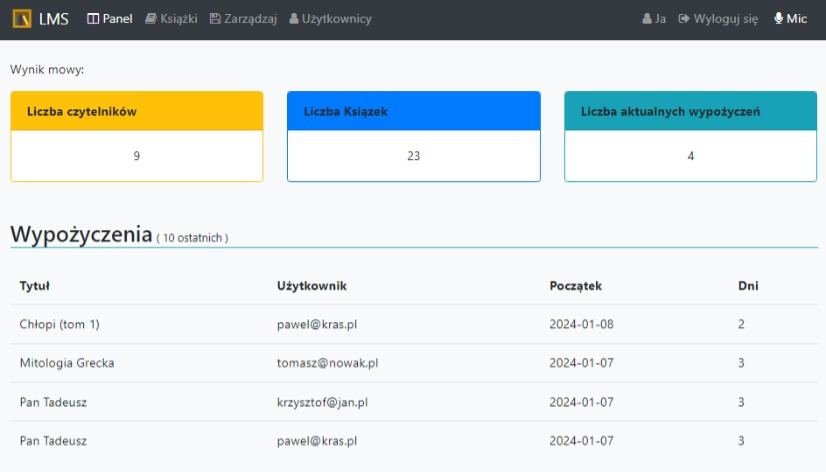
\includegraphics[width=0.75\textwidth]{images/gui}
    \captionsource{Interfejs graficzny w aplikacji}{Opracowanie własne}
    \label{fig:gui}
\end{figure}

\section{Interfejs głosowy}
Do obsługi interfejsu wykorzystano WebSpeechApi, który został wykorzystany w dwojaki sposób.\ Po pierwsze wykorzystano możliwości biblioteki do rozpoznawania i przetwarzania mowy.\ Dzięki temu po utworzeniu słownika słów kluczowych dostępnego dla aplikacji jest możliwe sterowanie większością funkcjonalności w sposób głosowy.\ Słownik ten został podany w \refsource{tabeli}{tab:keys}.\ Dodatkowo wykorzystane zostały możliwości syntezy mowy, które najlepiej zostały zobrazowane na formularzu dodawania nowych książek, gdzie po wysłaniu niepoprawnych danych aplikacja zwraca się do użytkownika, opisując mu jakie błędy popełnił.

\begin{table}[H]
    \centering
    \captionsource{Słownik słów kluczowych}{Opracowanie własne}
    \label{tab:keys}
\begin{tabular}{|c|c|c|c|} \hline
    \multicolumn{4}{|c|}{\textbf{Słownik słów kluczowych}} \\ \hline
    login & hasło & zaloguj się & ja \\ \hline
    wyloguj się & użytkownicy & zarządzaj & książki \\ \hline
    panel & dodaj & dodaj nową & dodaj nową książkę \\ \hline
    dodaj nowego & tytuł & autor & wiek \\ \hline
    granica wieku & zapisz & powrót & książka \\ \hline
    usuń & dodaj kopię & edytuj książkę & wypożycz \\ \hline
    użytkownik & oddaj & imię & nazwisko \\ \hline
    email & data & wyszukaj & indeks \\ \hline
    index & & & \\ \hline
\end{tabular}
\end{table}

Kod do obsługi tego interfejsu został w pełni napisany w języku Java Script.\ Kod opisany we fragmencie~\ref{frag:l2} Przedstawia wstępną konfigurację biblioteki WebSpeechApi, która jest wykorzystywana w projekcie.\ Powyższe fragmenty kodu przedstawiają kod napisany w języku JavaScript, którego oddziaływania na interfejs graficzny zostały opisane w części dokumentacji użytkowej, gdzie wskazywane są poszczególne funkcjonalności.

\lstinputlisting[language=HTML, caption={Konfiguracja WebSpeechApi}, label=frag:l2]{lang2.js}

Za rozpoznawanie i przetwarzanie słów na cyfry odpowiada metoda zawarta we fragmencie~\ref{frag:l1}.
\lstinputlisting[language=HTML, caption={Metoda zamieniająca słowa na cyfry}, label=frag:l1]{lang1.js}

Kod ukazany we fragmencie~\ref{frag:l5} odpowiada za konfigurację wydarzeń na stronie, które uruchamiają i wyłączają nasłuchiwanie.\ Dodatkowo odpowiada za obsłużenie wydarzeń biblioteki.\ Wydarzenia obsługiwane to:
\begin{itemize}
\item nomatch - nie rozpoznano mowy
\item speechend - wykryto koniec mowy
\item error - inny błąd
\end{itemize}

\lstinputlisting[language=HTML, caption={Obsługa wydarzeń związanych z mową}, label=frag:l5]{lang5.js}

Fragment kodu~\ref{frag:l3} odpowiada za wykorzystanie rezultatu przetwarzania mowy na tekst i obsłużenie różnych akcji m.in. uzupełniania formularzy.

\lstinputlisting[language=HTML, caption={Obsługa rezultatu rozpoznawania mowy}, label=frag:l3]{lang3.js}

Ostatni fragment~\ref{frag:l4} obsługuje słownik słów kluczowych na stronie, wykonując odpowiednie akcje przypisane do poszczególnych słów.

\lstinputlisting[language=HTML, caption={Obsługa słów kluczowych}, label=frag:l4]{lang4.js}